%!TEX program = xelatex
%!TEX options=--shell-escape
\documentclass[12pt]{article}

%
\usepackage[scheme=plain]{ctex}
%
\usepackage{fontspec}
%
\usepackage[margin = 1in]{geometry}

%
\usepackage[dvipsnames]{xcolor}
\usepackage[many]{tcolorbox}

%
\usepackage{amsmath}
\usepackage{amssymb}
\usepackage{amsthm}
%
\usepackage{tensor}
%
\usepackage{slashed}
\usepackage{physics}
\usepackage{simpler-wick}

%
\usepackage[version=4]{mhchem}

%
\usepackage{mathtools}

%
\usepackage{bm}
\newcommand{\dbar}{\dif\hspace*{-0.18em}\bar{}\hspace*{0.2em}}
\DeclareMathAlphabet\mathbfcal{OMS}{cmsy}{b}{n}
%\usepackage{bbold}
\newcommand*{\dif}{\mathop{}\!\mathrm{d}}
\newcommand*{\euler}{\mathrm{e}}
\newcommand*{\imagi}{\mathrm{i}}

\renewcommand{\vec}[1]{\boldsymbol{\mathbf{#1}}}

\usepackage{caption}
\usepackage{multirow}
\usepackage{enumitem}

%
\usepackage{mathrsfs}
\usepackage{dsfont}

%
\usepackage{hyperref}
\hypersetup{
    colorlinks=true,
    linkcolor=violet,
    filecolor=blue,      
    urlcolor=blue,
    citecolor=cyan,
}

%
\usepackage{graphicx}
\usepackage{subfig}
%
\graphicspath{{figures/}{../figures/}}


%
\usepackage{indentfirst}
%
\setlength{\parindent}{2em}
\linespread{1.25}

% 
% \setmainfont{Times New Roman}

\title{Note}
\author{Feng-Yang Hsieh}
\date{}

\begin{document}
\maketitle

\section{CWoLa}% (fold)
\label{sec:cwola}
	The Classification Without Labels (CWoLa) is a weakly supervised learning method. The CWoLa approach trains a model to discriminate the mixed samples, which are mixtures of the original signal and background samples. The optimal classifier in the CWoLa approach is also the optimal classifier in the traditional fully-supervised case where all label information is available. This section utilizes the CWoLa approach to train classifiers on di-Higgs samples.

	\subsection{Sample}% (fold)
	\label{sub:sample}
		This exercise's signal corresponds to the resonant Higgs boson pairs production in the four-$b$ quarks channel. These Higgs boson pairs are produced via gluon-gluon fusion in the two Higgs doublet model (2HDM). The Higgs boson $h$ ($m_h = \text{125 GeV}$) pair is produced by the heavy CP-even scalar $H$ with mass $m_H$ ranging from $\text{300 GeV}$ to $\text{1200 GeV}$. The background consists of QCD multi-jet events.

		The CWoLa training samples $M_1$ and $M_2$ are the mixtures of the signal and background samples. The probability distribution of the mixed sample is a combination of the signal $p_s(x)$ and background $p_B(x)$ distributions:
		\begin{equation}
			\begin{aligned}
				p_{M_1}(x) &=  f_1 p_S(x) + (1-f_1) p_B(x) \\
				p_{M_2}(x) &=  f_2 p_S(x) + (1-f_2) p_B(x)
			\end{aligned}
		\end{equation}
		where $f_1, f_2$ are the signal fractions, and $x$ represents the observables used for the classification task.

		DNN and SPANet network architectures are considered in this exercise. For DNN, the input features are summarised in Table \ref{tab:DNN_variables}, consisting of 16 variables. For SPANet, the input features are a list of final jets, each represented by their 4-momentum $(p_\text{T}, \eta,\phi, M)$ and a boolean $b$-tag.
		\begin{table}[htpb]
			\centering
			\caption{Input variables used to train the dense neural network.}
			\label{tab:DNN_variables}
			\begin{tabular}{l|c|c}
				Reconstructed objects       & Variables used for training   & \# \\ \hline
				Higgs candidate             & $(p_\text{T}, \eta, \phi, m)$ & 8  \\
				Subjets                     & $\Delta R(j_1,j_2)$                    & 2  \\
				b-tagging                   & Boolean for $j_i \in h_{1,2}^{\text{cand}}$       & 4  \\
				Di-Higgs system             & $p_\text{T}^{hh}, m_{hh}$        & 2 
			\end{tabular}		
		\end{table}

	% subsection sample (end)
	\subsection{Result}% (fold)
	\label{sub:result}
		The CWoLa training utilizes samples with different signal fractions $f_1,f_2$ to train the classifiers. The results of CWoLa training are shown in Figure~\ref{fig:CWoLa_training_result} with different signal fractions. When $f_1$ is far from $0.5$, the results tend to approach those of the fully supervised case.
		\begin{figure}[htpb]
			\centering
			\subfloat[DNN]{
				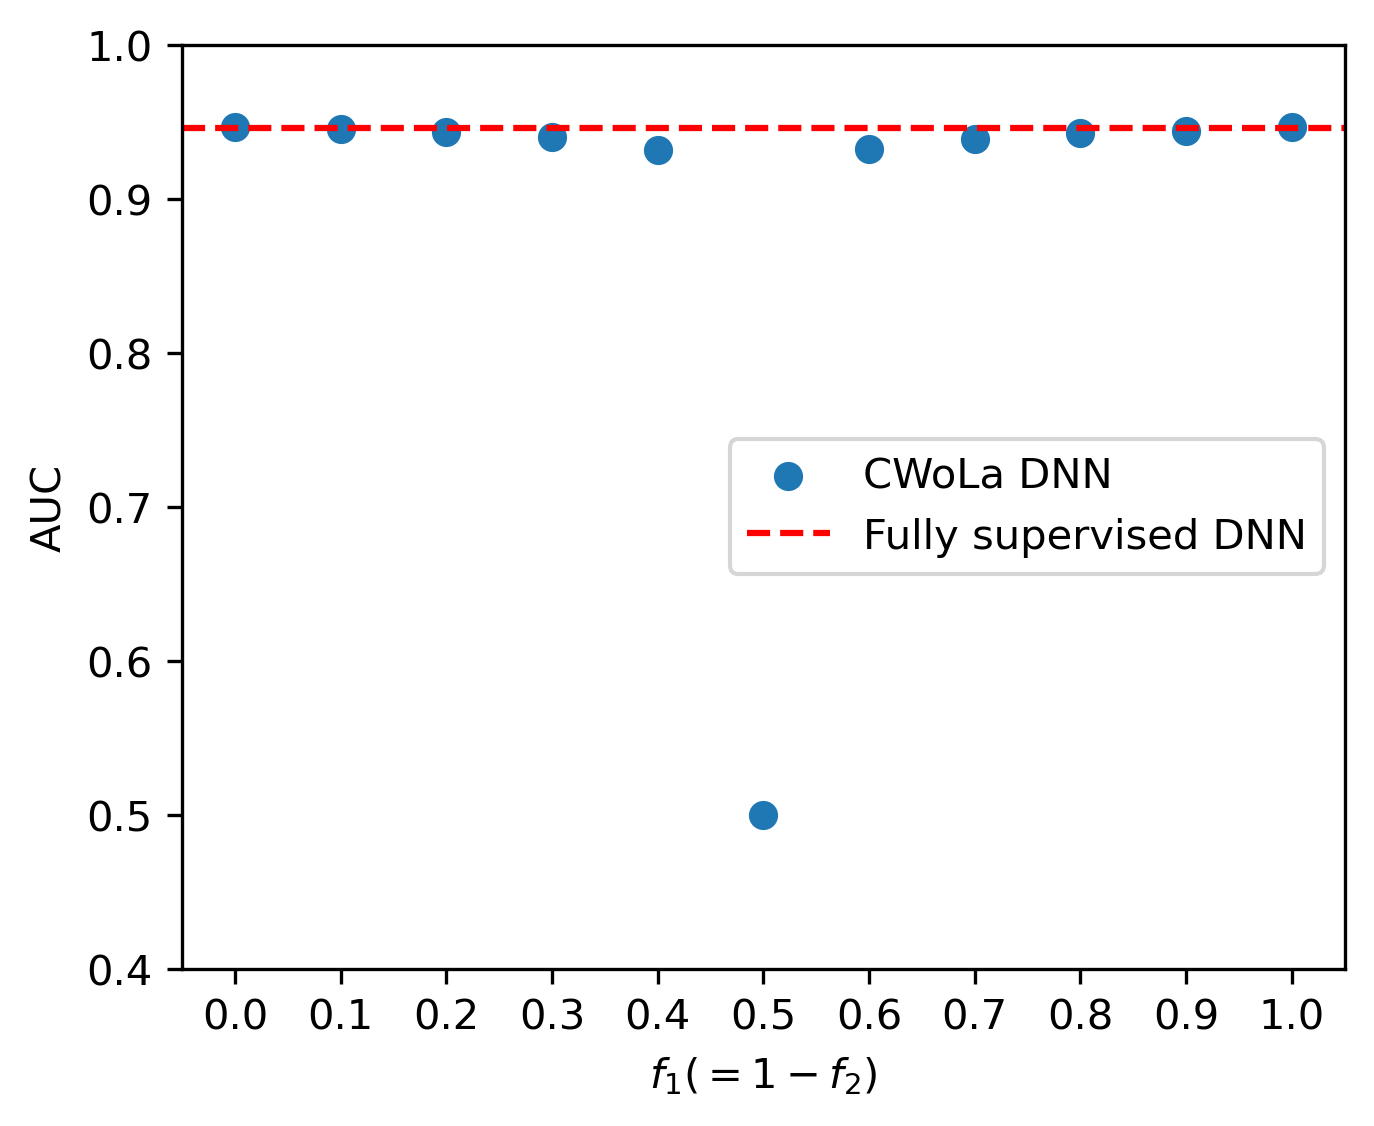
\includegraphics[width=0.45\textwidth]{CWoLa_DNN.png}
			}
			\subfloat[SPANet]{
				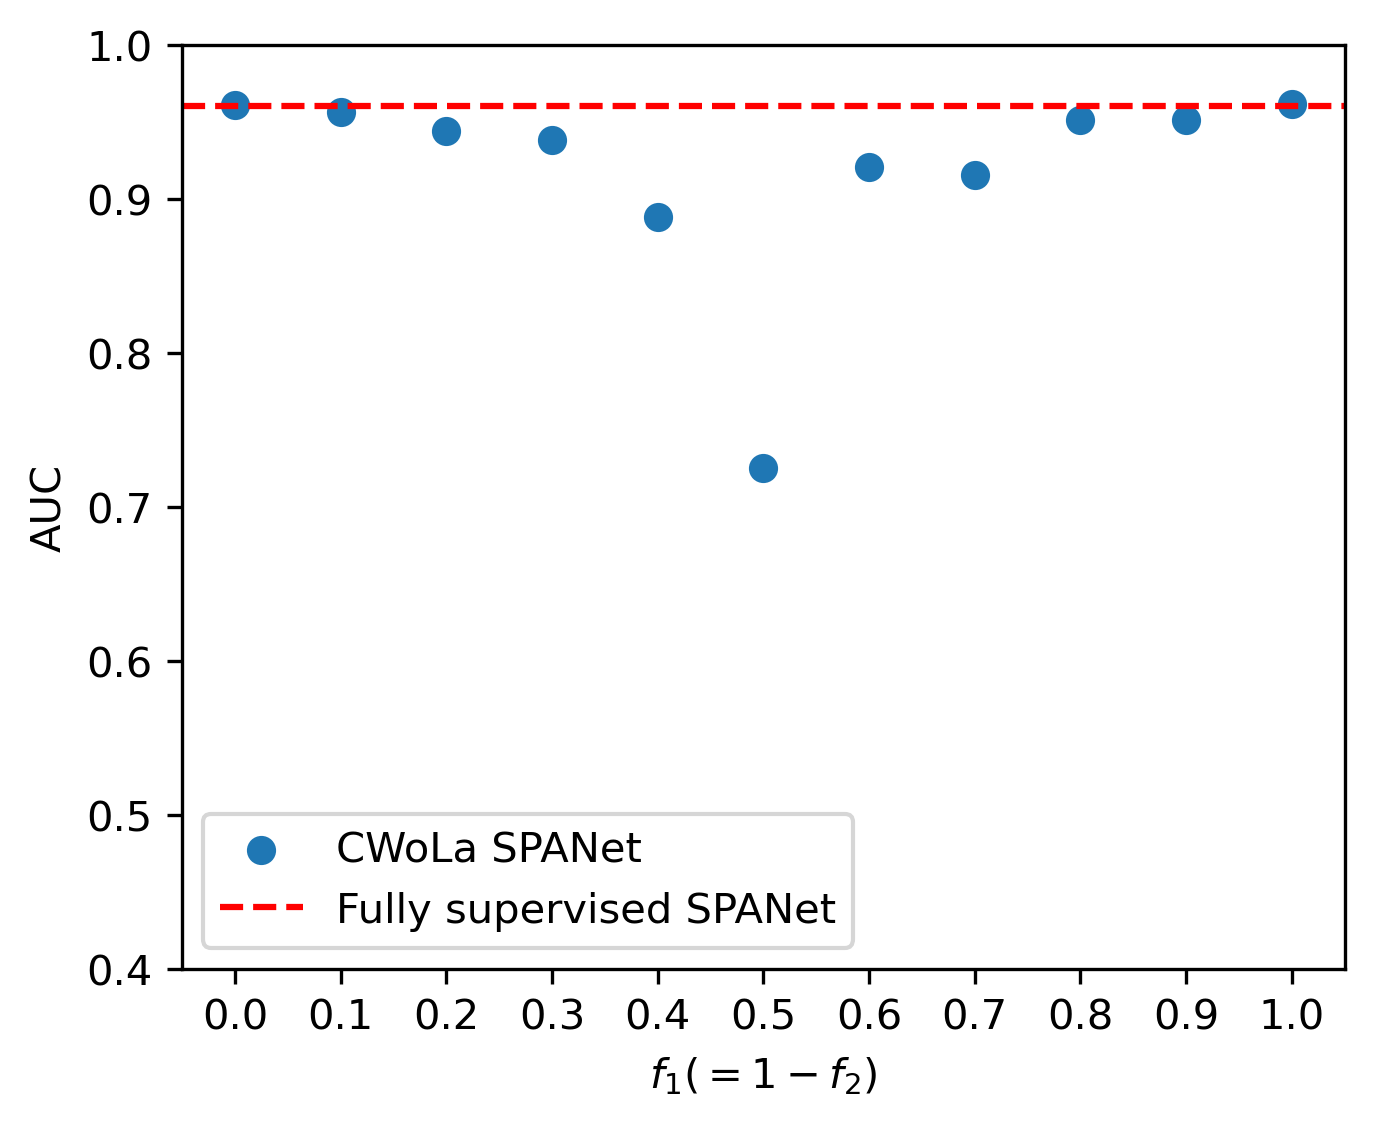
\includegraphics[width=0.45\textwidth]{CWoLa_SPANet.png}
			}
			\caption{The AUC of CWoLa training as a function of the signal fraction $f_1$. For simplicity, we set signal fraction $f_2$ equal to $1 - f_1$. The horizontal dashed line indicates the fully-supervised AUC.}
			\label{fig:CWoLa_training_result}
		\end{figure}

		When $f_1 = 0.5$ the mixed sample $M_1$ and $M_2$ have identical distributions, so the classifier can not learn anything in this case. In the case of DNN, the AUC is $0.5$, as expected. However, for SPANet, the AUC is more than $0.7$.

		This is because SPANet is trained on both pairing and classification tasks simultaneously. The pairing part introduces some asymmetries between signal and background samples, leading to the AUC that deviates from $0.5$.

		To investigate the effect of the pairing task on SPANet's performance, the weight of the pairing component is set to zero, meaning that SPANet focuses solely on the classification task. Figure~\ref{fig:CWoLa_SPANet_without_pairing} shows the SPANet training results without pairing task. In this case, as expected, the AUC is close to $0.5$ when $f_1 = 0.5$. 
		\begin{figure}[htpb]
			\centering
			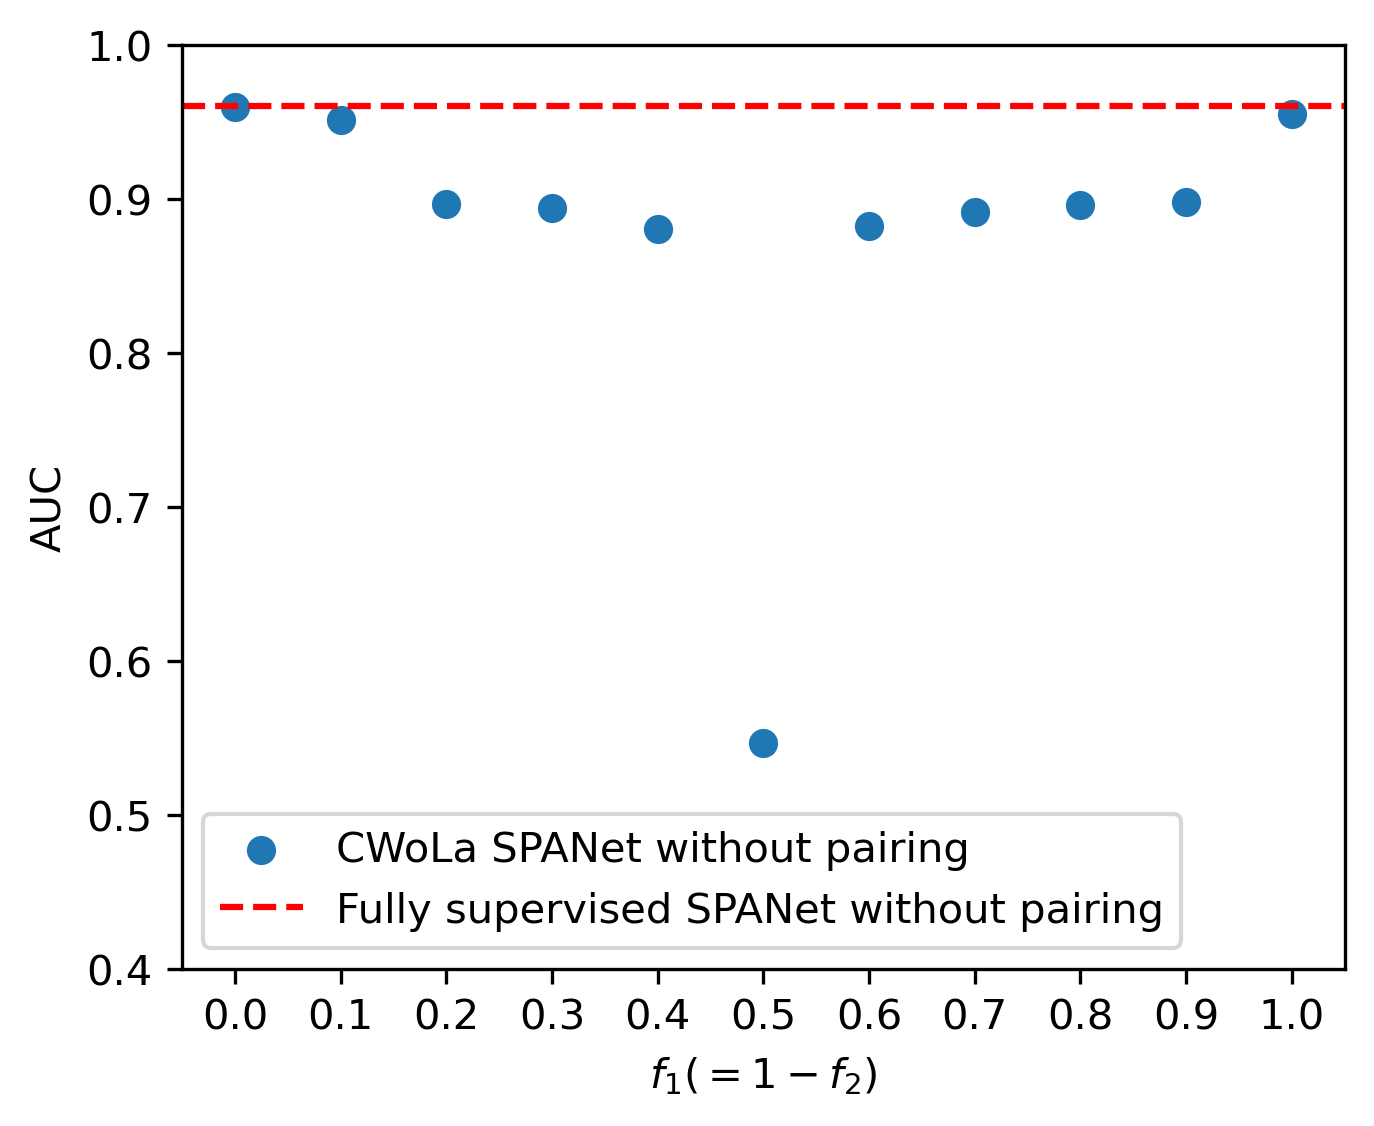
\includegraphics[width=0.65\textwidth]{CWoLa_SPANet_no_pair.png}
			\caption{The AUC of CWoLa SPANet training as a function of the signal fraction $f_1$. For simplicity, we set signal fraction $f_2$ equal to $1 - f_1$. Here, SPANet is trained on the classification task only.}
			\label{fig:CWoLa_SPANet_without_pairing}
		\end{figure}	
	% subsection result (end)	
% section cwola (end)

\section{CWoLa hunting}% (fold)
\label{sec:cwola_hunting}
	\subsection{Sample}% (fold)
	\label{sub:sample_cwola_hunting}
		The signal is the resonant Higgs boson pairs production in the four-$b$ quarks channel. In this section, the Higgs boson pair is produced by the heavy CP-even scalar $H$ with mass $m_H = \text{1000 GeV}$. The background consists of QCD multi-jet events. The basic requirement is the ``four-tag cut,'' which requires at least four $b$-tagged $R = 0.4$ anti-$k_t$ jets with $p_\text{T} > \text{40 GeV}$ and $\abs{\eta} < 2.5$. Only the events passing the four-tag cut are used in the following analysis.
		
		The CWoLa hunting approach utilizes the signal region and sideband region to create the mixed training sample. The total invariant mass $m_{hh}$ of the di-Higgs system is utilized to determine the signal and sideband region. This quantity is computed from the four $b$-jets with the highest transverse momentum. Figure~\ref{fig:mhh_distribution} presents the $m_{hh}$ distribution of signal and background samples. The signal region is $[800, 1050] \text{ GeV}$ and the sideband region is $[700, 800]\cup [1050, 1100] \text{ GeV}$. This signal and sideband region are chosen such that the corresponding cross-sections are closed.
		\begin{figure}[htpb]
			\centering
			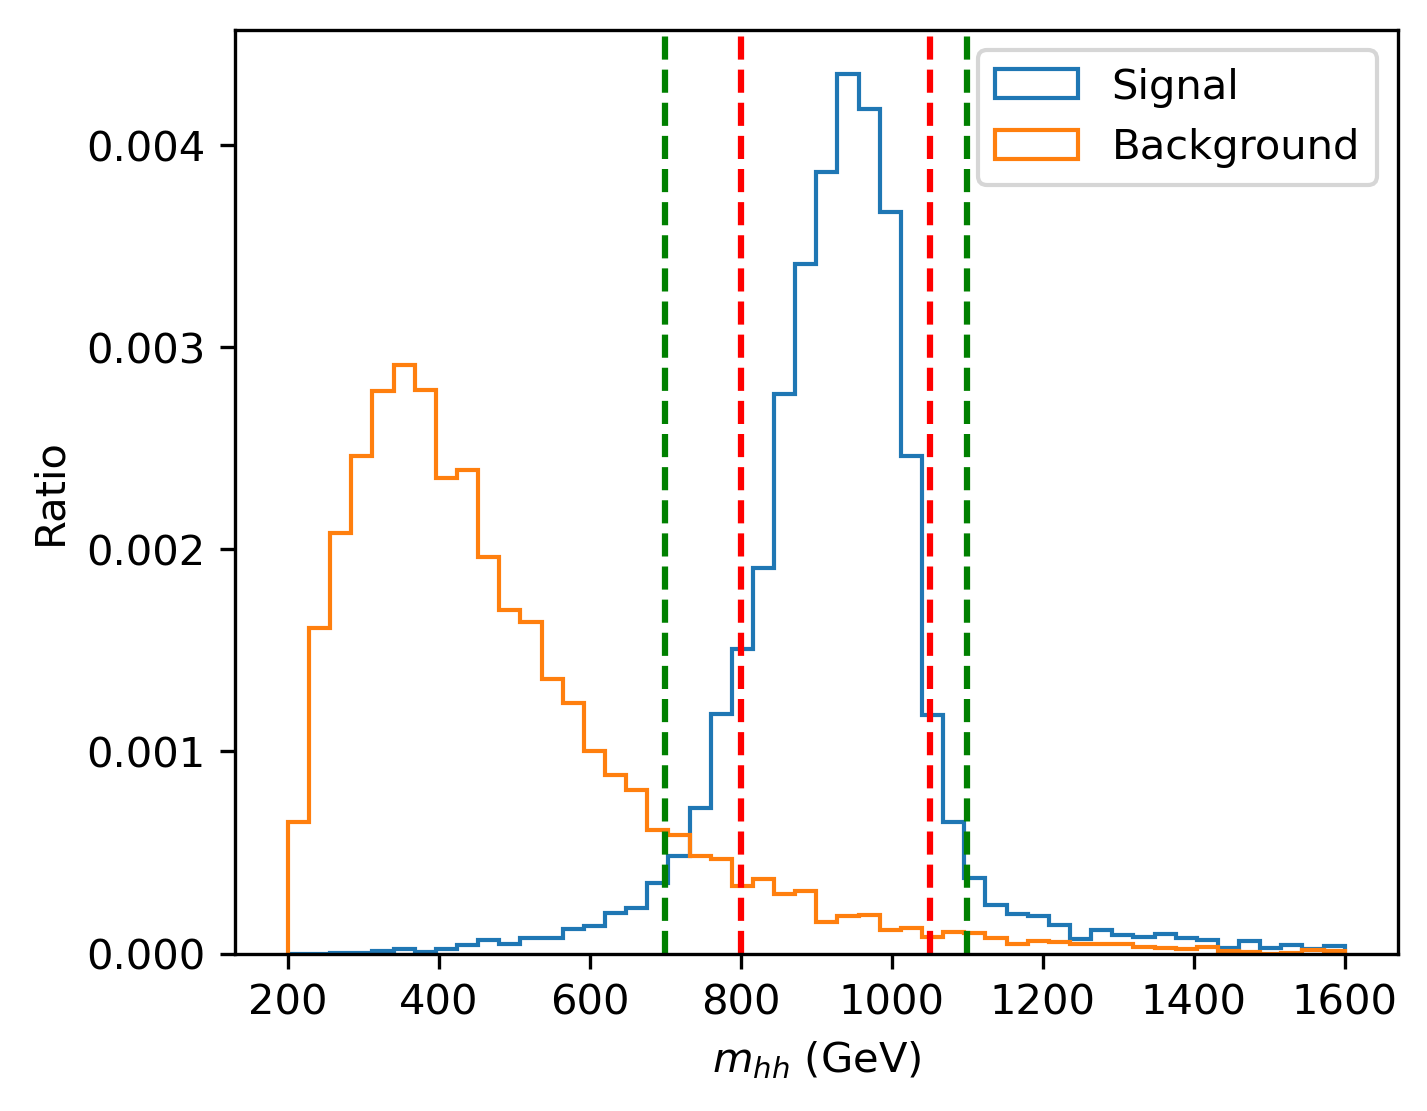
\includegraphics[width=0.65\textwidth]{mhh_distribution.png}
			\caption{The totoal invriant mass $m_{hh}$ distribution of signal and background samples. The signal region is $[800, 1050] \text{ GeV}$ between the red dashed lines. The sideband region is $[700, 800]\cup [1050, 1100] \text{ GeV}$ between the green dashed lines and exclude the signal region.}
			\label{fig:mhh_distribution}
		\end{figure}

		Table~\ref{tab:diHiggs_cutflow_table} is the cutflow table of the selection cuts. The number of events used in mixed training samples could be computed from these cross-sections. The training sample size is presented in Table~\ref{tab:training_sample_size_cwola_hunting}.
		\begin{table}[htpb]
			\centering
			\caption{The cross sections for the di-Higgs signal and background processes at different selection cuts.}
			\label{tab:diHiggs_cutflow_table}
			\begin{tabular}{l|cc|c|c}
								& \multicolumn{2}{c|}{Cross section (fb)} &          & $\mathcal{L} = 139 \text{ fb}^{-1}$ \\
								& Signal           & Background           & $S / B$  & $S/\sqrt{B}$                        \\ \hline
				Four tag        & 0.081            & 6.03e+03             & 1.34e-05 & 0.0123                              \\ \hline
				Signal region   & 0.063            & 3.32e+02             & 1.90e-04 & 0.0408                              \\
				Sideband region & 0.010            & 3.19e+02             & 3.03e-05 & 0.0064                             
			\end{tabular}
		\end{table}
		\begin{table}[htpb]
			\centering
			\caption{The training sample size for the mixed sample. The luminosity is $\mathcal{L} = 78 \text{ fb}^{-1}$ because the generated samples are not enough for now.}
			\label{tab:training_sample_size_cwola_hunting}
			
			\begin{tabular}{c|cc}
							 & \multicolumn{2}{c}{True label} \\
				Mixed sample & Signal       & Background      \\ \hline
				$M_1$            & 5            & 26k             \\
				$M_2$            & 1            & 25k            
			\end{tabular}
		\end{table}

		Consider the DNN CWoLa classifier. The Higgs candidates are reconstructed by the $\text{min-}\Delta R$ pairing method. The input features are similar to the previous case (Table~\ref{tab:DNN_variables}), but the $b$-tagging information and total invariant mass of the di-Higgs system are excluded. For $\text{min-}\Delta R$ pairing, it only uses the $b$-tagged jets. Total invariant mass is already used to determine the signal and sideband region.

	% subsection sample_cwola_hunting (end)
	\subsection{Training results}% (fold)
	\label{sub:training_results}
		Table \ref{tab:cwola_hunting_DNN_results} presents the DNN classification training results. These numbers are evaluated from the pure samples. The training datasets with and without signal events have similar results. This suggests that the DNN fails to distinguish the signal and background samples but learns the difference between the signal and sideband region. Moreover, the results also imply the input features may correlate to the total invariant mass of the di-Higgs system.
		\begin{table}[htpb]
			\centering
			\caption{The CWoLa DNN training results. The average and standard deviation of 10 training are presented.}
			\label{tab:cwola_hunting_DNN_results}
			\begin{tabular}{c|cc}
				& ACC     & AUC   \\ \hline
				With signal   & $0.868 \pm 0.024$ & $0.925 \pm 0.023$ \\
				No signal     & $0.850 \pm 0.033$ & $0.909 \pm 0.026$
			\end{tabular}      
		\end{table}

		Figure~\ref{fig:signal_score_distribution} shows the signal score distributions. Even though the signal scores are very different for signal and background distributions, the difference probably stems from the $m_{hh}$ distribution.
	 	\begin{figure}[htpb]
			\centering
			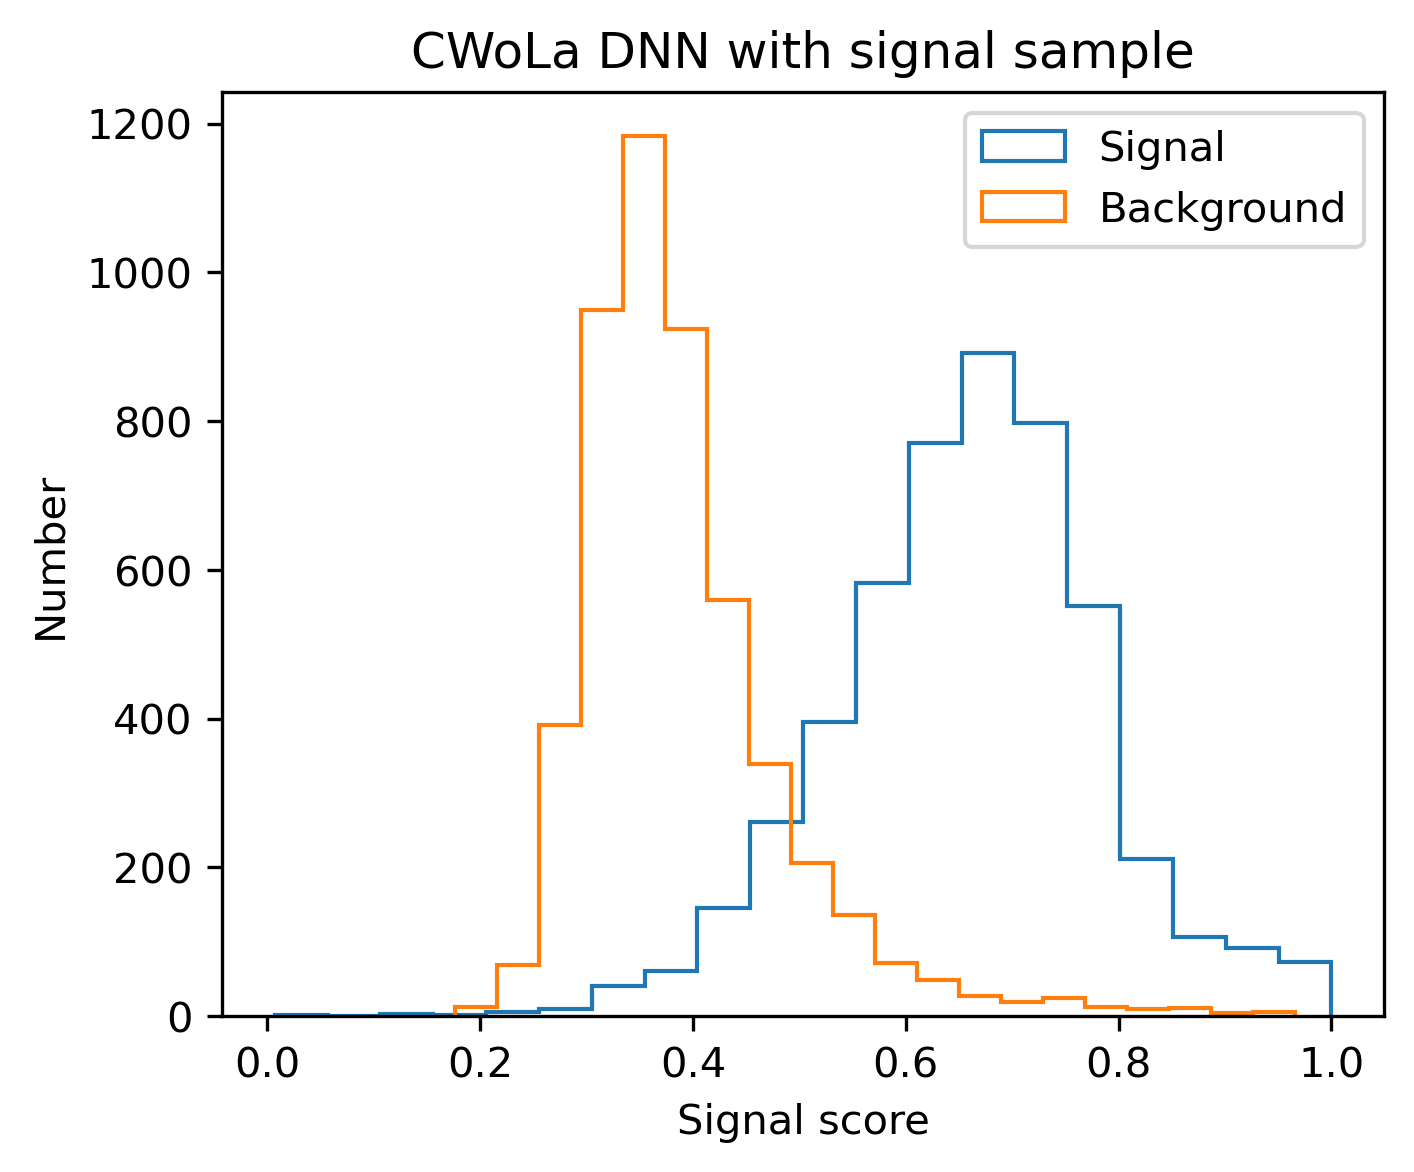
\includegraphics[width=0.45\textwidth]{DNN_w_sig_signal_score_distribution.png}
			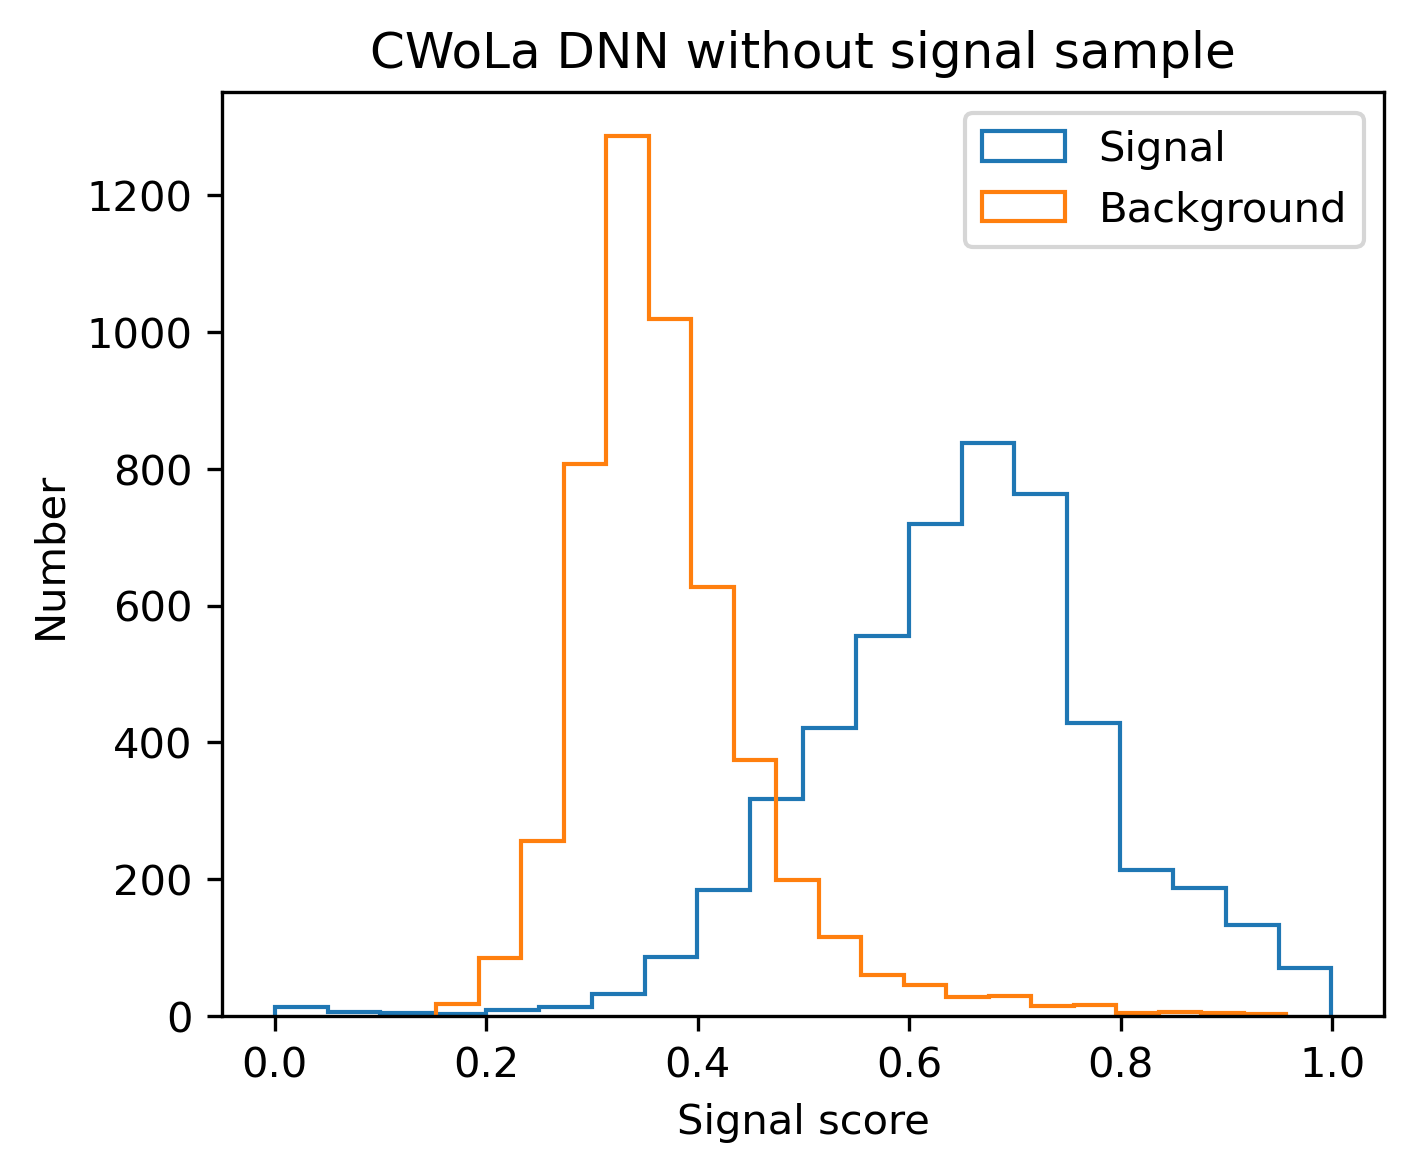
\includegraphics[width=0.45\textwidth]{DNN_wo_sig_signal_score_distribution.png}
			\caption{The signal score distributions. We apply the CWoLa DNN on pure samples to obtain the signal score distributions.}
			\label{fig:signal_score_distribution}
		\end{figure}

		There are two issues:
		\begin{itemize}
			\item The input features might correlated to the observables used to determine the signal and sideband region. We need to construct other independent input variables.
			\item The signal fraction is too low. It is hard to learn something about signal events. 
		\end{itemize}
	% subsection training_results (end)
% section cwola_hunting (end)		
\end{document} 

